% GNUPLOT: LaTeX picture with Postscript
\begingroup
  \makeatletter
  \providecommand\color[2][]{%
    \GenericError{(gnuplot) \space\space\space\@spaces}{%
      Package color not loaded in conjunction with
      terminal option `colourtext'%
    }{See the gnuplot documentation for explanation.%
    }{Either use 'blacktext' in gnuplot or load the package
      color.sty in LaTeX.}%
    \renewcommand\color[2][]{}%
  }%
  \providecommand\includegraphics[2][]{%
    \GenericError{(gnuplot) \space\space\space\@spaces}{%
      Package graphicx or graphics not loaded%
    }{See the gnuplot documentation for explanation.%
    }{The gnuplot epslatex terminal needs graphicx.sty or graphics.sty.}%
    \renewcommand\includegraphics[2][]{}%
  }%
  \providecommand\rotatebox[2]{#2}%
  \@ifundefined{ifGPcolor}{%
    \newif\ifGPcolor
    \GPcolortrue
  }{}%
  \@ifundefined{ifGPblacktext}{%
    \newif\ifGPblacktext
    \GPblacktextfalse
  }{}%
  % define a \g@addto@macro without @ in the name:
  \let\gplgaddtomacro\g@addto@macro
  % define empty templates for all commands taking text:
  \gdef\gplbacktext{}%
  \gdef\gplfronttext{}%
  \makeatother
  \ifGPblacktext
    % no textcolor at all
    \def\colorrgb#1{}%
    \def\colorgray#1{}%
  \else
    % gray or color?
    \ifGPcolor
      \def\colorrgb#1{\color[rgb]{#1}}%
      \def\colorgray#1{\color[gray]{#1}}%
      \expandafter\def\csname LTw\endcsname{\color{white}}%
      \expandafter\def\csname LTb\endcsname{\color{black}}%
      \expandafter\def\csname LTa\endcsname{\color{black}}%
      \expandafter\def\csname LT0\endcsname{\color[rgb]{1,0,0}}%
      \expandafter\def\csname LT1\endcsname{\color[rgb]{0,1,0}}%
      \expandafter\def\csname LT2\endcsname{\color[rgb]{0,0,1}}%
      \expandafter\def\csname LT3\endcsname{\color[rgb]{1,0,1}}%
      \expandafter\def\csname LT4\endcsname{\color[rgb]{0,1,1}}%
      \expandafter\def\csname LT5\endcsname{\color[rgb]{1,1,0}}%
      \expandafter\def\csname LT6\endcsname{\color[rgb]{0,0,0}}%
      \expandafter\def\csname LT7\endcsname{\color[rgb]{1,0.3,0}}%
      \expandafter\def\csname LT8\endcsname{\color[rgb]{0.5,0.5,0.5}}%
    \else
      % gray
      \def\colorrgb#1{\color{black}}%
      \def\colorgray#1{\color[gray]{#1}}%
      \expandafter\def\csname LTw\endcsname{\color{white}}%
      \expandafter\def\csname LTb\endcsname{\color{black}}%
      \expandafter\def\csname LTa\endcsname{\color{black}}%
      \expandafter\def\csname LT0\endcsname{\color{black}}%
      \expandafter\def\csname LT1\endcsname{\color{black}}%
      \expandafter\def\csname LT2\endcsname{\color{black}}%
      \expandafter\def\csname LT3\endcsname{\color{black}}%
      \expandafter\def\csname LT4\endcsname{\color{black}}%
      \expandafter\def\csname LT5\endcsname{\color{black}}%
      \expandafter\def\csname LT6\endcsname{\color{black}}%
      \expandafter\def\csname LT7\endcsname{\color{black}}%
      \expandafter\def\csname LT8\endcsname{\color{black}}%
    \fi
  \fi
    \setlength{\unitlength}{0.0500bp}%
    \ifx\gptboxheight\undefined%
      \newlength{\gptboxheight}%
      \newlength{\gptboxwidth}%
      \newsavebox{\gptboxtext}%
    \fi%
    \setlength{\fboxrule}{0.5pt}%
    \setlength{\fboxsep}{1pt}%
\begin{picture}(5668.00,5668.00)%
    \gplgaddtomacro\gplbacktext{%
    }%
    \gplgaddtomacro\gplfronttext{%
      \csname LTb\endcsname%%
      \put(1085,690){\makebox(0,0){\strut{}\num{300}}}%
      \put(1814,690){\makebox(0,0){\strut{}\num{350}}}%
      \put(2543,690){\makebox(0,0){\strut{}\num{400}}}%
      \put(3271,690){\makebox(0,0){\strut{}\num{450}}}%
      \put(4000,690){\makebox(0,0){\strut{}\num{500}}}%
      \put(4729,690){\makebox(0,0){\strut{}\num{550}}}%
      \put(2834,360){\makebox(0,0){\strut{}$x$ (\si{mm})}}%
      \put(601,1304){\makebox(0,0)[r]{\strut{}\num{220}}}%
      \put(601,1714){\makebox(0,0)[r]{\strut{}\num{240}}}%
      \put(601,2124){\makebox(0,0)[r]{\strut{}\num{260}}}%
      \put(601,2534){\makebox(0,0)[r]{\strut{}\num{280}}}%
      \put(601,2944){\makebox(0,0)[r]{\strut{}\num{300}}}%
      \put(601,3354){\makebox(0,0)[r]{\strut{}\num{320}}}%
      \put(601,3764){\makebox(0,0)[r]{\strut{}\num{340}}}%
      \put(601,4174){\makebox(0,0)[r]{\strut{}\num{360}}}%
      \put(601,4584){\makebox(0,0)[r]{\strut{}\num{380}}}%
      \put(7,2944){\rotatebox{-270}{\makebox(0,0){\strut{}$y$ (\si{mm})}}}%
      \put(5313,997){\makebox(0,0)[l]{\strut{}\num{-1}}}%
      \put(5313,1970){\makebox(0,0)[l]{\strut{}\num{-0.5}}}%
      \put(5313,2944){\makebox(0,0)[l]{\strut{}\num{0}}}%
      \put(5313,3917){\makebox(0,0)[l]{\strut{}\num{0.5}}}%
      \put(5313,4891){\makebox(0,0)[l]{\strut{}\num{1}}}%
    }%
    \gplbacktext
    \put(0,0){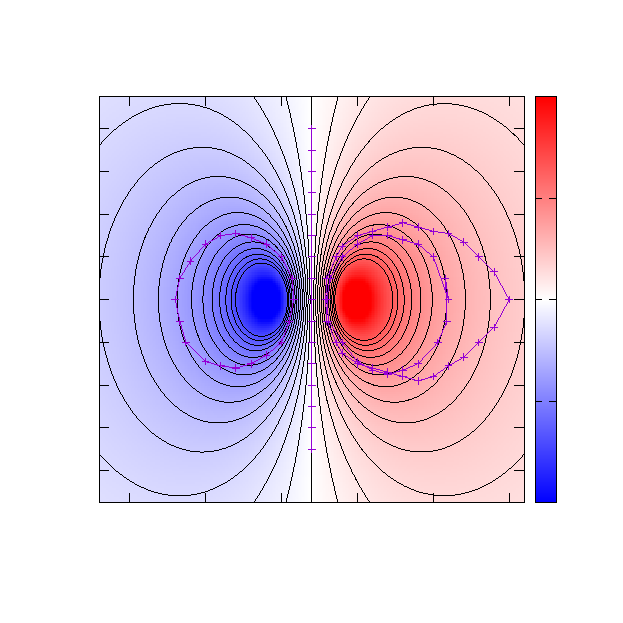
\includegraphics{fils}}%
    \gplfronttext
  \end{picture}%
\endgroup
